\section{Введение}

Хорошо известно, что теория аттракторов динамических систем не обеспечивает нахождение глобальных аттракторов
большого числа уравнений и систем.
В связи с этим появились новые подходы к понятию глобальных аттракторов дифференциальных уравнений.
Один из таких подходов основан на теории траекторных аттракторов (см. \cite{Chepyzhov, Sell, Vorotnikov2, Zvyagin}),
в которой глобальный аттрактор системы является сечением соответствующего минимального траекторного аттрактора.
Одним из препятствий для широкого применения этого подхода (в частности, для уравнений гидродинамики)
является требование инвариантности траекторного пространства относительно операторов сдвига
$T(t)$, $T(t)u(s) = u(s+t)$, $t\geq 0$.
В \cite{Vorotnikov2, Zvyagin} удалось отказаться от этого требования,
но при этом траекторные аттракторы могли состоять  не только из решений соответствующей системы (см. \cite{Sell5}),
хотя минимальный траекторный аттрактор, сечение которого в этой теории является глобальным аттрактором,
всегда может быть аппроксимирован сдвигами траекторий по времени (теорема 4.2.5, стр. 92 \cite{Zvyagin}).
Этот эффект проявляется уже на уровне динамических систем, а именно,
в силу единственности решения задачи Коши динамику уравнения можно описать в терминах полугрупп,
однако иногда оказывается, что соответствующая полугруппа не имеет глобального аттрактора.
Однако может оказаться,
что если подходить к описанию динамики этой системы с точки зрения глобального аттрактора пространства траекторий,
то глобальный аттрактор существует
и является сечением не только подмножества решений.
Ниже приводится пример
системы, для которой минимальный траекторный аттрактор целиком лежит вне пространства траекторий этой системы
и для которого существует глобальный аттрактор в смысле
аттрактора траекторных пространств,
но аттракторов в смысле динамических систем не существует.

\section{}
Рассмотрим разбиение  $\mathbb{R}^2$ на пять непересекающихся связных множеств следующим образом:
$$
	A_0 = \{ (x_1, x_2) \mid 0 < x_1 < 1, 0 < x_2 < 1\},
$$
$$
	A_1 = \{ (x_1, x_2) \mid x_1 < 1, x_2 \leq 0  \},
	A_2 = \{ (x_1, x_2) \mid x_1 \geq 1, x_2 < 1  \},
$$
$$
	A_3 = \{ (x_1, x_2) \mid x_1 > 0, x_2 \geq 1  \},
	A_4 = \{ (x_1, x_2) \mid x_1 \leq 0, x_2 > 0  \}
$$
и отметим точки
$\alpha_1=(1, 0)$,
$\alpha_2=(1, 1)$,
$\alpha_3=(0, 1)$ и
$\alpha_4=\alpha_0=(0, 0)$
(последнее двойное обозначение используется для удобства работы с индексами).
Разбиение плоскости показано на рис. \ref{fig:somelabel}.

\begin{figure}[h]
	\centering
	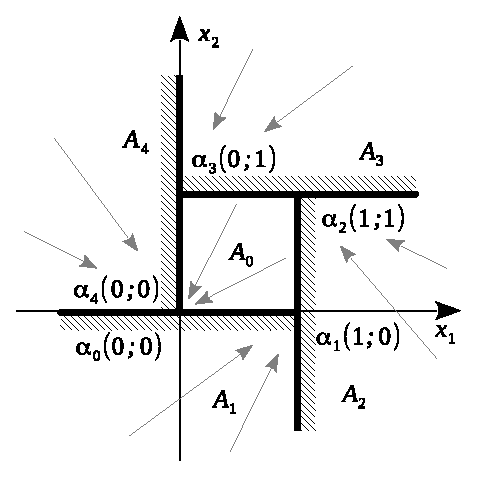
\includegraphics[width=0.4\linewidth]{quad3.eps}
	\caption{Разбиение плоскости, отмеченные точки и направления сдвигов}
	\label{fig:somelabel}
	%\vspace{2cm}
\end{figure}

Сразу заметим, что $\alpha_i \in \overline{A_i}$, $i=0,...,4$ и
$\alpha_i \in A_{i+1}$, $i=0,...,3$ (тогда как $\alpha_4 = \alpha_0 \in A_{1}$).

Таким образом, вся координатная плоскость оказалась разбита на четыре угла $A_1, ..., A_4$ и квадрат $A_0$.
Квадрат не включает свои границы; для каждого угла одна его сторона включается в угол,
а вторая сторона и вершина --- нет (они включаются в <<соседний>> угол).
Именно за счёт такого разбиения и достигается эффект примера.

В дальнейшим в случае, когда нижних индексов два, первый нижний индекс
будет отвечать за номер области и обозначаться через $i$,
$i=0, ..., 4$, второй --- за номер координаты
(или соответствующего ей уравнения) и обозначаться $j$, $j=1, 2$.

Рассмотрим систему двух обыкновенных дифференциальных уравнений
\begin{equation}\label{difur_primer_R2}
	\frac{dx_j(t)}{dt} = -c_{ij} \cdot (x_j(t)-\alpha_{ij})^2, \mbox{~~} j=1,2, \mbox{~~} i=0,...,4
\end{equation}
если
$
	(x_1, x_2) \in A_i,  \alpha_i = (\alpha_{i1},\alpha_{i2}),
$
$i=0,...,4$,
где
$
	c_{ij} = \operatorname{sgn}(x_j(0)-\alpha_{ij}),
$
если $x_j(0) - \alpha_{ij} \neq 0$,
и $c_{ij} = 0$ в противном случае.
Обратим внимание, что каждая координата точки траектории меняется независимо от другой,
и далее будет показано, что она стремится
к некоторому предельному значению.

Говоря подробнее,
$c_{ij}$ обращается в ноль только на границах углов $A_i$ и только для одной координаты на каждом луче,
образующем эти границы.
Например, на открытом луче, исходящем из точки $\alpha_2=(1, 1)$ вниз и включенном в угол $A_2$, система (\ref{difur_primer_R2})
принимает вид:
\begin{equation*}
	\begin{cases}
		\dfrac{dx_1(t)}{dt} = 0, &\mbox{(т.к. $x_1(0) = 1 = \alpha_{21}$, имеем $c_{21} = 0$)}
	\\\\
		\dfrac{dx_2(t)}{dt} =  (x_2(t)-1)^2,  &\mbox{(т.к. $x_2(0) < 1 = \alpha_{22}$, имеем $c_{22} = -1$)}
	\end{cases}
\end{equation*}
Во внутренних точках угла $A_2$, т.е. не лежащих на этом луче, имеем:
$x_1(0) - \alpha_{21} = x_1(0) - 1 > 0$ и следовательно $c_{21} = 1$;
$x_2(0) - \alpha_{22} = x_2(0) - 1 < 0$ и следовательно $c_{22} = -1$.
Таким образом, во внутренности угла $A_2$ система (\ref{difur_primer_R2})
принимает вид:
\begin{equation*}
	\begin{cases}
		\dfrac{dx_1(t)}{dt} =  - (x_1(t)-1)^2
	\\\\
		\dfrac{dx_2(t)}{dt} =  (x_2(t)-1)^2.
	\end{cases}
\end{equation*}

Вернёмся к общему виду системы (\ref{difur_primer_R2}).
Для $c_{ij} \neq 0$ решения системы (\ref{difur_primer_R2}) на $[0, \infty)$ имеют вид
\begin{equation}\label{primer_R2_x_j}
	x_j(t) = \frac{c_{ij}}{t+C_0}+\alpha_{ij}, C_0 > 0,
\end{equation}
откуда
$
	x_j(t) \xrightarrow[t\to \infty ]{}{\alpha_{ij}},
$
при этом знак разности $x_j(t) - \alpha_{ij}$ не меняется (поскольку числитель дроби на зависит от $t$, а знаменатель всегда строго положителен).
Если же $c_{ij}=0$, то легко видеть, что $x_j(t) = x_j(0) = \alpha_{ij}$,
и формула (\ref{primer_R2_x_j}) также верна.

Выпишем теперь оператор сдвига.
Положим в (\ref{primer_R2_x_j}) $t=0$, получим
$
	x_j(0) = c_{ij}/{C_0}+\alpha_{ij}
$.

Выразив отсюда $C_0$, подставим его и $c_{ij}$ в (\ref{primer_R2_x_j}).
Таким образом, оператор сдвига по траекториям уравнения (\ref{difur_primer_R2}) имеет вид
\begin{equation}\label{primer_R2_oper_sdviga}
	\tilde{S}_t(x_{j}(0)) = \frac{x_{j}(0)-\alpha_{ij}}{|x_{j}(0)-\alpha_{ij}|t+1}+\alpha_{ij}
\end{equation}

Заметим, что числитель дроби не зависит от $t$, а знаменатель всегда строго положителен.
Следовательно, разность $\tilde{S}_t(x_j(0)) - \alpha_{ij}$ сохраняет знак,
и траектория, начавшись в области $A_i$, никогда не перейдёт в другую область $A_{i'}$, $i \neq i'$.

Для $x_0 \in A_i$ имеем
\begin{equation}\label{primer_R2_stremlenie}
	S_t(x_0) \xrightarrow[t \to \infty]{} \alpha_{i},
\end{equation}
причём монотонно по $t$.
Действительно,
\begin{multline}
	\|S_t(x_0) - \alpha_i\| \leq
	\sqrt{2} \max_{j=1,2} \left| \frac{x_{j}(0)-\alpha_{ij}}{|x_{j}(0)-\alpha_{ij}|t+1} + \alpha_{ij} - \alpha_{ij}  \right| =
	\sqrt{2} \max_{j=1,2} \left| \frac{x_{j}(0)-\alpha_{ij}}{|x_{j}(0)-\alpha_{ij}|t+1} \right| \leq
	\\ \leq
	\sqrt{2} \max_{j=1,2} \left| \frac{x_{j}(0)-\alpha_{ij}}{|x_{j}(0)-\alpha_{ij}|t} \right| =
	\sqrt{2} \max_{j=1,2} \left| \frac{1}{t} \right| =
	\frac{\sqrt{2}}{t} \xrightarrow[t \to \infty]{} 0
\end{multline}

Заметим, что эта оценка не зависит от начального условия.
Более того, из того, что $\alpha_i \in A_{i+1}$, $i=0,...,3$,
следует, что $S_t(\alpha_i) \xrightarrow[t \to \infty]{} \alpha_{i+1}$,
т.~е. множество функций-констант
$$
	U = \{ u_i(t) \equiv \alpha_i \}_{i=0}^{3}
$$
не пересекается со множеством решений уравнения (\ref{difur_primer_R2}).

Перейдём теперь к обсуждению аттракторов.
Дадим необходимые определения.
Пусть $E$ и $E_0$ --- банаховы пространства, $E$ рефлексивно,
$E_0 \subset E$, причём норма в $E_0$ не обязательно индуцирована нормой в $E$;
$F$~--- топологическое пространство, такое, что $E \cap F \ne \varnothing$.
Определения мы будем давать в общем виде, хотя в рассматриваемом примере
$E=E_0=F=\mathbb{R}^2$.

\begin{definition}
	Множество $\mathcal{H}^+$ называется трансляционно инвариантным, если
	для любого $t \geq 0$ выполнено $T(t)\mathcal{H}^+ \subset \mathcal{H}^+$,
	где $(T(h)f)(t)=f(t+h)$ для $f \in \mathcal{H}^+$.
\end{definition}


\begin{definition}
Пусть $B \subset T_+$.
Сечением множества траекторий $B$ в момент времени $t \geq 0$ называется множество
$
	B(t)=\left\{u(t) : u \in B \right\} \subset E.
$
\end{definition}


\begin{definition}
Пусть $R,Q \subset E_0$.
Полуотклонением в пространстве $E_0$ множества $R$ от множества $Q$ называется величина
$
	h_{E_0}(R,Q) = \sup_{r\in R} \inf_{q \in Q} \| q - r \|_{E_0}.
$
\end{definition}
Свойства полуотклонения подробно описаны в [\cite{mnogozn}, теорема 1.2.41].



\begin{definition}
Семейство отображений $S_t : E \to E$, $t \geq 0$ называется полугруппой трансляций,
если $S_0$ --- тождественное отображение и
$
	\forall(t>0,\tau>0)[S_t \circ S_\tau = S_{t+\tau}]
$
\end{definition}

\begin{definition}
Множество $A$ называется инвариантным относительно полугруппы трансляций $S_t$, если
$
	\forall(t\geq 0)[S_t A = A]
$
\end{definition}

\begin{definition}
Множество $P \subset F$ называется $(E,F)$-притягивающим для полугруппы трансляций $S_t$,
если для любого ограниченного множества $B \subset E$ и любой открытой окрестности $W$ множества $P$ в $F$ существует число $h\geq 0$ такое, что
$
	\forall(t \geq h)[S_t B \subset W]
$
\end{definition}


\begin{definition}
Множество $A\subset E\cap F$ называется $(E,F)$-аттрактором полугруппы трансляций (аттрактором динамической системы)  $S_t$, если

а) $A$ компактно в $F$ и ограничено в $E$;

б) $A$ инвариантно относительно полугруппы трансляций $S_t$.

в) $A$ является $(E,F)$-притягивающим для полугруппы трансляций $S_t$.

\end{definition}


\begin{definition}
	Множество $P \subset T_+$ называется притягивающим для пространства траекторий $\mathcal{H}^+$ в топологии пространства $C(\mathbb{R}_+; E_0)$,
	если для всякого множества $B \subset \mathcal{H}^+$, ограниченного в $L_{\infty}(\mathbb{R}_+;E)$, выполнено условие
	$
		h_{E_0}(B(t),T(t)P) \xrightarrow[t\to\infty]{}0
	$.
\end{definition}

\begin{definition}\label{def:traj_attr}
	Непустое множество $\mathcal{U}\subset T^+$
	называется траекторным аттрактором для пространства траекторий $\mathcal{H}^+$
	относительно топологии $C(\mathbb{R}_+,E_0)$, если
	%\begin{enumerate}
	%	\item
			$\mathcal{U}$ компактно в $C(\mathbb{R}_+,E_0)$,
			ограничено в $L_{\infty}(\mathbb{R}_+,E)$,
			трансляционно инвариантно
	%	\item
			и является притягивающим для пространства траекторий $\mathcal{H}^+$
			в топологии пространства $C(\mathbb{R}_+; E_0)$.
	%\end{enumerate}
\end{definition}

\begin{definition}
	Минимальным траекторным аттрактором пространства траекторий $\mathcal{H}^+$
	называется его минимальный по включению траекторный аттрактор.
\end{definition}

Покажем теперь, что $U$~--- траекторный аттрактор в смысле определения \ref{def:traj_attr}.


Компактность и ограниченность множества из четырёх функций-констант в пространствах
$C(\mathbb{R}_+; \mathbb{R}^2)$ и $L_\infty(\mathbb{R}_+; \mathbb{R}^2)$ очевидна.
Очевидно и то, что $U$ трансляционно инвариантно.
%
Осталось показать, что $U$ есть притягивающее множество в пространстве траекторий уравнения (\ref{difur_primer_R2}),
которое мы обозначим $H^+$.
Действительно, пусть $M>0$ и $B\subset H^+$ --- ограниченное в $L_\infty(\mathbb{R}_+; \mathbb{R}^2)$ множество.
Тогда
\begin{multline*}
	h_{C([0,M];\mathbb{R}^2)}(\Pi_M T(t)B,\Pi_M U) =
	\sup_{v\in B} \inf_{u\in U} \| T(t) v - u \|_{C([0,M];\mathbb{R}^2)} =
	\\ =
	\sup_{v\in B} \min_{i=0,..,3} \| T(t) v - u_i \|_{C([0,M];\mathbb{R}^2)} =
	\sup_{v\in B} \min_{i=0,..,3} \max_{s\in[0,M]} \| (T(t) v)(s) - u_i(s) \| =
	\\ =
	\sup_{v\in B} \min_{i=0,..,3} \max_{s\in[0,M]} \| (T(t) v)(s) - \alpha_i \| =
	\sup_{v\in B} \min_{i=0,..,3} \max_{s\in[t,t+M]} \| v(s) - \alpha_i \| \leq
	\frac{\sqrt{2}}{t} \xrightarrow[t\to + \infty]{} 0
\end{multline*}
Таким образом, $U$ --- действительно траекторный аттрактор, пересечение которого с пространством траекторий
уравнения (\ref{difur_primer_R2}) пусто.
Минимальный траекторный аттрактор содержится в любом траекторном аттракторе, в частности, в $U$,
следовательно, минимальный траекторный аттрактор в данном случае целиком лежит вне пространства траекторий
(и можно доказать, что он в точности равен $U$).

\section{}

Покажем теперь, что глобального аттрактора полугруппы трансляций
в смысле динамической системы в данном примере не существует.
Предположим противное, т.е. что существует $P$ --- глобальный аттрактор полугруппы трансляций,
порождаемой оператором сдвига (\ref{primer_R2_oper_sdviga}).

Пусть сначала $\alpha_i \notin P$ для некоторого $i=0,...,4$.
В силу определения глобального аттрактора полугруппы трансляций,
$P$ компактно в $\mathbb{R}^2$.
Тогда расстояние $\rho$ от $P$ до $\alpha_i$ положительно.

Положим $\varepsilon = {\rho}/{3} > 0$ и покажем,
что условие притяжения из определения аттрактора полугруппы трансляций не выполняется.

Рассмотрим $V_\varepsilon = A_i \cap B(\alpha_i, \varepsilon)$ и некоторое решение $x_\varepsilon(t)$
такое, что $x_\varepsilon(0) \in V_\varepsilon$.
Тогда в силу монотонности стремления (\ref{primer_R2_stremlenie})
$x_\varepsilon(t) \in V_\varepsilon, t>0$.
Но $V_\varepsilon$ отделено от $P$, следовательно, $x_\varepsilon{t}$ не попадает в $\varepsilon$--окрестность $P$
ни при каких положительных $t$, что доказывает нарушение условия притяжения.

Значит, если аттрактор $P$ полугруппы трансляций существует, то $\alpha_i \in P, i=0,...,4$.
Но тогда $S_t P \ne P, t>0$.
Действительно, траектория, выходящая из $\alpha_i$, стремится к $\alpha_{i+1}$;
а все траектории, выходящие из точек области $A_i$, стремятся к $\alpha_i$,
но никогда не достигают её,
т.е. при выходе из нуля точка $\alpha_i$ <<выпадает>> из аттрактора $P$, чего быть не должно.

Следовательно, аттрактора полугруппы трансляций в данном случае не существует.
